\documentclass[aspectratio=169,12pt]{beamer}
\usetheme{Warsaw}
\usecolortheme{rose}
\usepackage[utf8]{inputenc}
\usepackage[T2A]{fontenc}
\usepackage[russian]{babel}
\usepackage{amssymb}
\usepackage{amsmath}
\usepackage{listings}
\title{Приложение для чтения новостей с linux.org.ru}
\subtitle{https://github.com/AlexanderTitilin/lor\_reader}
\author{Титилин Александр}
\institute{СПбГЭУ}
\date{}
\begin{document}
\begin{frame}
    \titlepage
\end{frame}
\begin{frame}
    \frametitle{Возможности программы}
    \begin{itemize}
        \item Получение всех новостей по тегу
        \item Получение всех новостей по тегу за опредеделенный период
        \item Сохранение новостей
    \end{itemize}
\end{frame}
\begin{frame}
    \frametitle{Пример работы программы}
    \begin{columns}
        \begin{column}{0.34\textwidth}
            Получение всех новостей с тегом "python"
        \end{column}
        \begin{column}{0.56 \textwidth}
            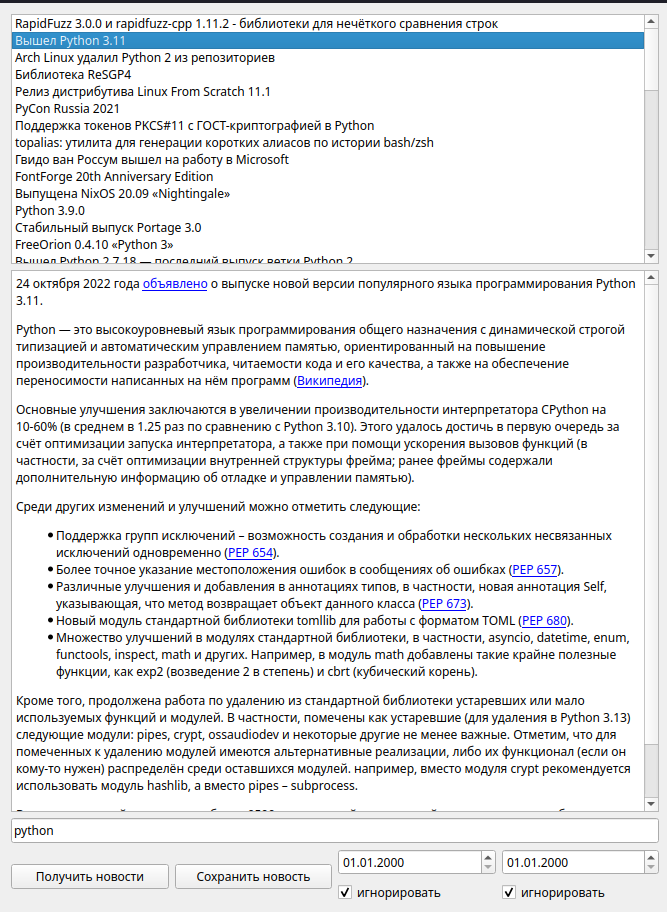
\includegraphics[width = \textwidth,height=220]{python1.png}
        \end{column}
    \end{columns}
\end{frame}
\begin{frame}
    \frametitle{Пример работы программы}
    \begin{columns}
        \begin{column}{0.34\textwidth}
            Получение всех новостей с тегом "java", созданных раньше 01.01.2008.
        \end{column}
        \begin{column}{0.56 \textwidth}
            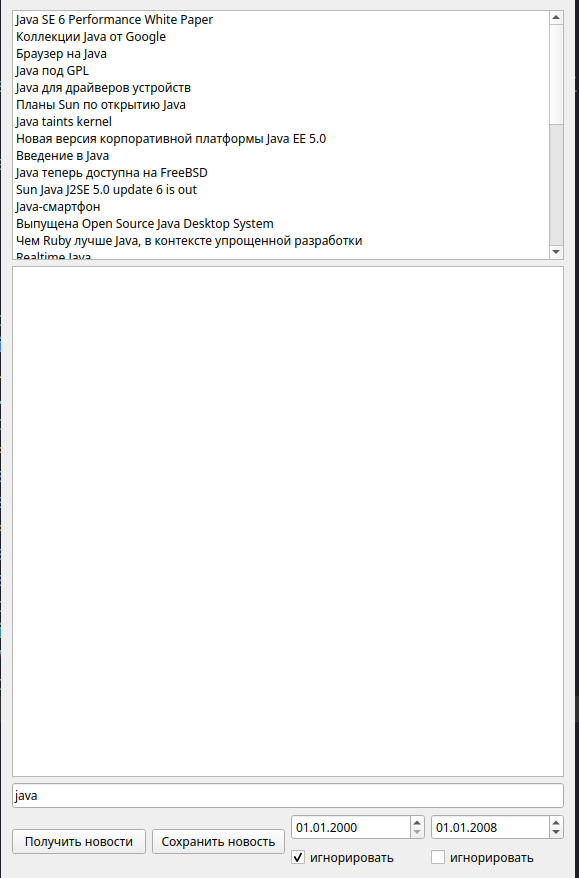
\includegraphics[width = \textwidth,height=220]{java2008.png}
        \end{column}
    \end{columns}
\end{frame}
\begin{frame}
    \frametitle{Использованные модули}
    \begin{itemize}
        \item PySide6 для создания графического интерфейса.
        \item Requests для  http-запросов.
        \item BeautifulSoup для парсинга html.
        \item Datetime для работы с датами.
        \item re
        \item itertools
        \item Dataclasses
        \item sys
    \end{itemize}
\end{frame}
\begin{frame}
    \frametitle{Использованное программное обеспечение}
    \begin{enumerate}
        \item neovim -- текстовый редактор
        \item latex для создания презентации
    \end{enumerate}
\end{frame}
\begin{frame}
    \frametitle{Вывод}
    Доделать можно многое
    \begin{enumerate}
        \item новые сайты для чтения новостей
        \item другие библиотеки для интерфейса
    \end{enumerate}
\end{frame}
\end{document}

